\documentclass[12pt,a4paper,xcolor=dvipsnames]{beamer}
%\usepackage[utf8x]{inputenc}
%\usepackage{ucs}
\usepackage[ansinew]{inputenc} % Kodierung
\usepackage{ngerman} % Sprache
\usepackage{amsmath}
\usepackage{amsfonts}
\usepackage{amssymb}
\usepackage{graphicx}
\usepackage{wrapfig}
\usepackage{verbatim}
\usepackage{xcolor}

%\usetheme{Frankfurt}
\setbeamertemplate{navigation symbols}{}

\title{Konflikthandhabung\\Theorie und Praxis}
\author{Robin Ellerkmann, Sven Reber}
\date{4. Februar 2017}

% Uebersicht
%//Folien zu einzelnen F�hrungsstilen
%//Withdrawing, inaction: Robin
%//Others: Sven

%//Jeder remote sein Zeug
%//Fazit Folie


\begin{document}
\maketitle

%\frame{\frametitle{Inhaltsverzeichnis}\tableofcontents}

\section{Willkommenin der Psychologie}
\begin{frame}
	%\frametitle{Willkommen}
	\center\huge{Willkommen\\in den Wissenschaften}
	\pause
	\center\huge{der \textbf{Psychologie}}
\end{frame}


\section{Einleitung und Definition}
\begin{frame}
	\frametitle{Inhalt}
	
	% FIXME: am Ende noch mal dem "echten" Inhalt/Titeln anpassen.
	\begin{itemize}
		\item Einleitung und Definition eines Konfliktes		% Sven
		\item Vergleich der Modelle					% Robin
		\begin{itemize}
			\item Prozessmodell
			\item Strukturmodell
		\end{itemize}
		\item F�hrungsstile							% Sven (ersten 3), Robin (widh-drawing, inaction)
		% XXX: F�r den Inahlt vllt. doch etwas zu viel/fr�h. "Erschl�gt" vllt. etwas. (Sven)		
		%\begin{itemize}
		%	\item Vermeidung (in-action)				% Robin
		%	\item Machteinsatz						% Sven
		%	\item Kompromiss						% Sven
		%	\item Anpassung (with-drawing)				% Robin
		%	\item Zusammenarbeit (problem solving)		% Sven
		%\end{itemize}
		\item Fazit									% Robin (?)
	\end{itemize}
\end{frame}

\section{Vergleich der Modelle}
\begin{frame}
	\frametitle{Modelle der Konflikthandhabung}
	\begin{itemize}
		\item Modellieren Konfliktverhalten zwischen zwei Parteien
		\item Zwei Ans\"atze:
		\begin{itemize}
			\item Prozessmodell
			\item Strukturmodell
		\end{itemize}
	\end{itemize}
\end{frame}

\subsection{Prozessmodell}
\begin{frame}
	\frametitle{Prozessmodell}
	\begin{itemize}
		\item Beschreibt interne Dynamik eines Konfliktes als Ablauf von Phasen
		\item Events identifizieren und deren Bedeutung f\"ur weitere Events ermitteln
		\item Dyadische Konflikte laufen in Eventzyklen ab
	\end{itemize}
\end{frame}

\begin{frame}
	\frametitle{Abbildung Prozessmodell}
% TODO: Temporary removed. Include in final again!!! (Sven)
\begin{center}$<$BILD: Prozessmodell$>$\end{center}
%	\begin{figure}[p]
%		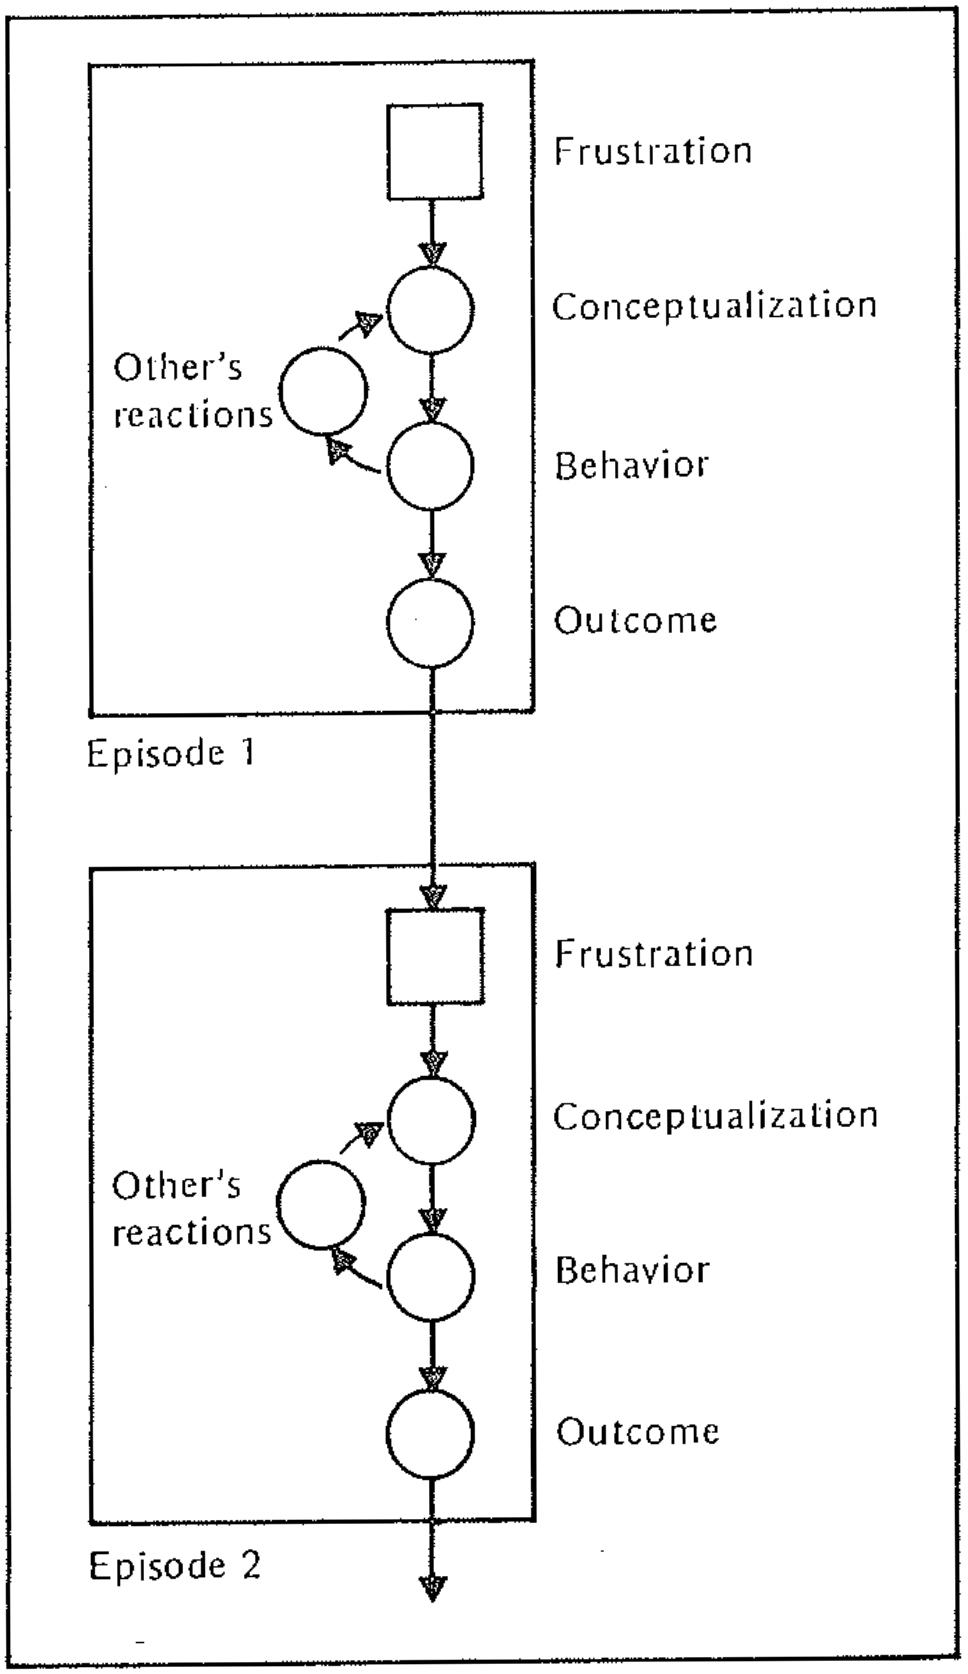
\includegraphics[width=0.4\textwidth]{images/process_model.png}
%	\end{figure}
\end{frame}

\begin{frame}
	\frametitle{Frustration}
	\begin{itemize}
		\item Ausgangspunkt f\"ur Konflikte: Frustration bei einer der Parteien
		\item Frustration kann viele Formen haben
	\end{itemize}
\end{frame}

\begin{frame}
%//TODO: Adjust name
	\frametitle{Wahrnehmung}
	\begin{itemize}
		\item Subjektive Definition des Anliegens f\"ur beide Parteien
		\item Drei Dimensionen bestimmen diese Definition:
		\begin{itemize}
			\item Egozentrik
			\item Einblick in zugrundeliegende Belange
			%\item Gr\"oße/Wichtigkeit des Problems
			\item Gr��e\,/\,Wichtigkeit des Problems
		\end{itemize}
		\item Bewusstsein \"uber m\"ogliche Handlungen und deren Folgen ist begrenzt
	\end{itemize}
\end{frame}

\begin{frame}
	\frametitle{Verhalten}
	\begin{itemize}
		\item Besteht aus drei Komponenten: Orientierung, strategische Ziele und Taktiken
		\item Orientierung: Wie wichtig ist einer Partei die Er\"ullung des eigenen Anliegens? Wie wichtig ist die Er\"ullung des Anliegens der anderen Partei?
		\item Strategische Ziele: Anpassung der Verhaltensweisen an den Gegen\"uber
		\item Taktiken: Beschreiben bestimmte Verhaltensweisen der Parteien. Z.\,B. als Wettbewerbstaktik, Kooperative Taktik, Bargaining Taktik
	\end{itemize}
\end{frame}

\begin{frame}
	\frametitle{Interaktion}
	\begin{itemize}
		\item Zwei Perspektiven: Verhaltensweisen sind selbst gew�hlt oder Verhaltensweisen werden durch Aktionen der anderen Partei ausgel\"ost
		\item Selbst gew�hltes Verhalten: Ver�nderung der Wahrnehmung des Konflikts �ndert Verhalten
		\item Ausgel\"ostes Verhalten: Resultiert aus psychologischen Dynamiken, z.\,B. Eskalation\,/\,Deeskalation
	\end{itemize}
\end{frame}

\begin{frame}
	\frametitle{Ergebnis}
	\begin{itemize}
		\item Nachwirkungen des Konflikts
		\item Langzeiteffekte 
	\end{itemize}
\end{frame}

\subsection{Strukturmodell}
\begin{frame}
	\frametitle{Strukturmodell}
	\begin{itemize}
		\item Identifiziert Parameter, die das Konfliktverhalten der Parteien beeinflussen
		\item Drei Arten von Einfluss auf das Konfliktverhalten jeder Partei:
		\begin{itemize}
			\item Verhaltensabsichten der Partei
			\item Sozialer Druck auf die Partei
			\item Beziehung zwischen den Interessen der Parteien
		\end{itemize}
	\end{itemize}
\end{frame}

\begin{frame}
	\frametitle{Abbildung Strukturmodell}
% TODO: Temporary removed. Include in final again!!! (Sven)
\begin{center}$<$BILD: Strukturmodell$>$\end{center}
%	\begin{figure}[p]
% 		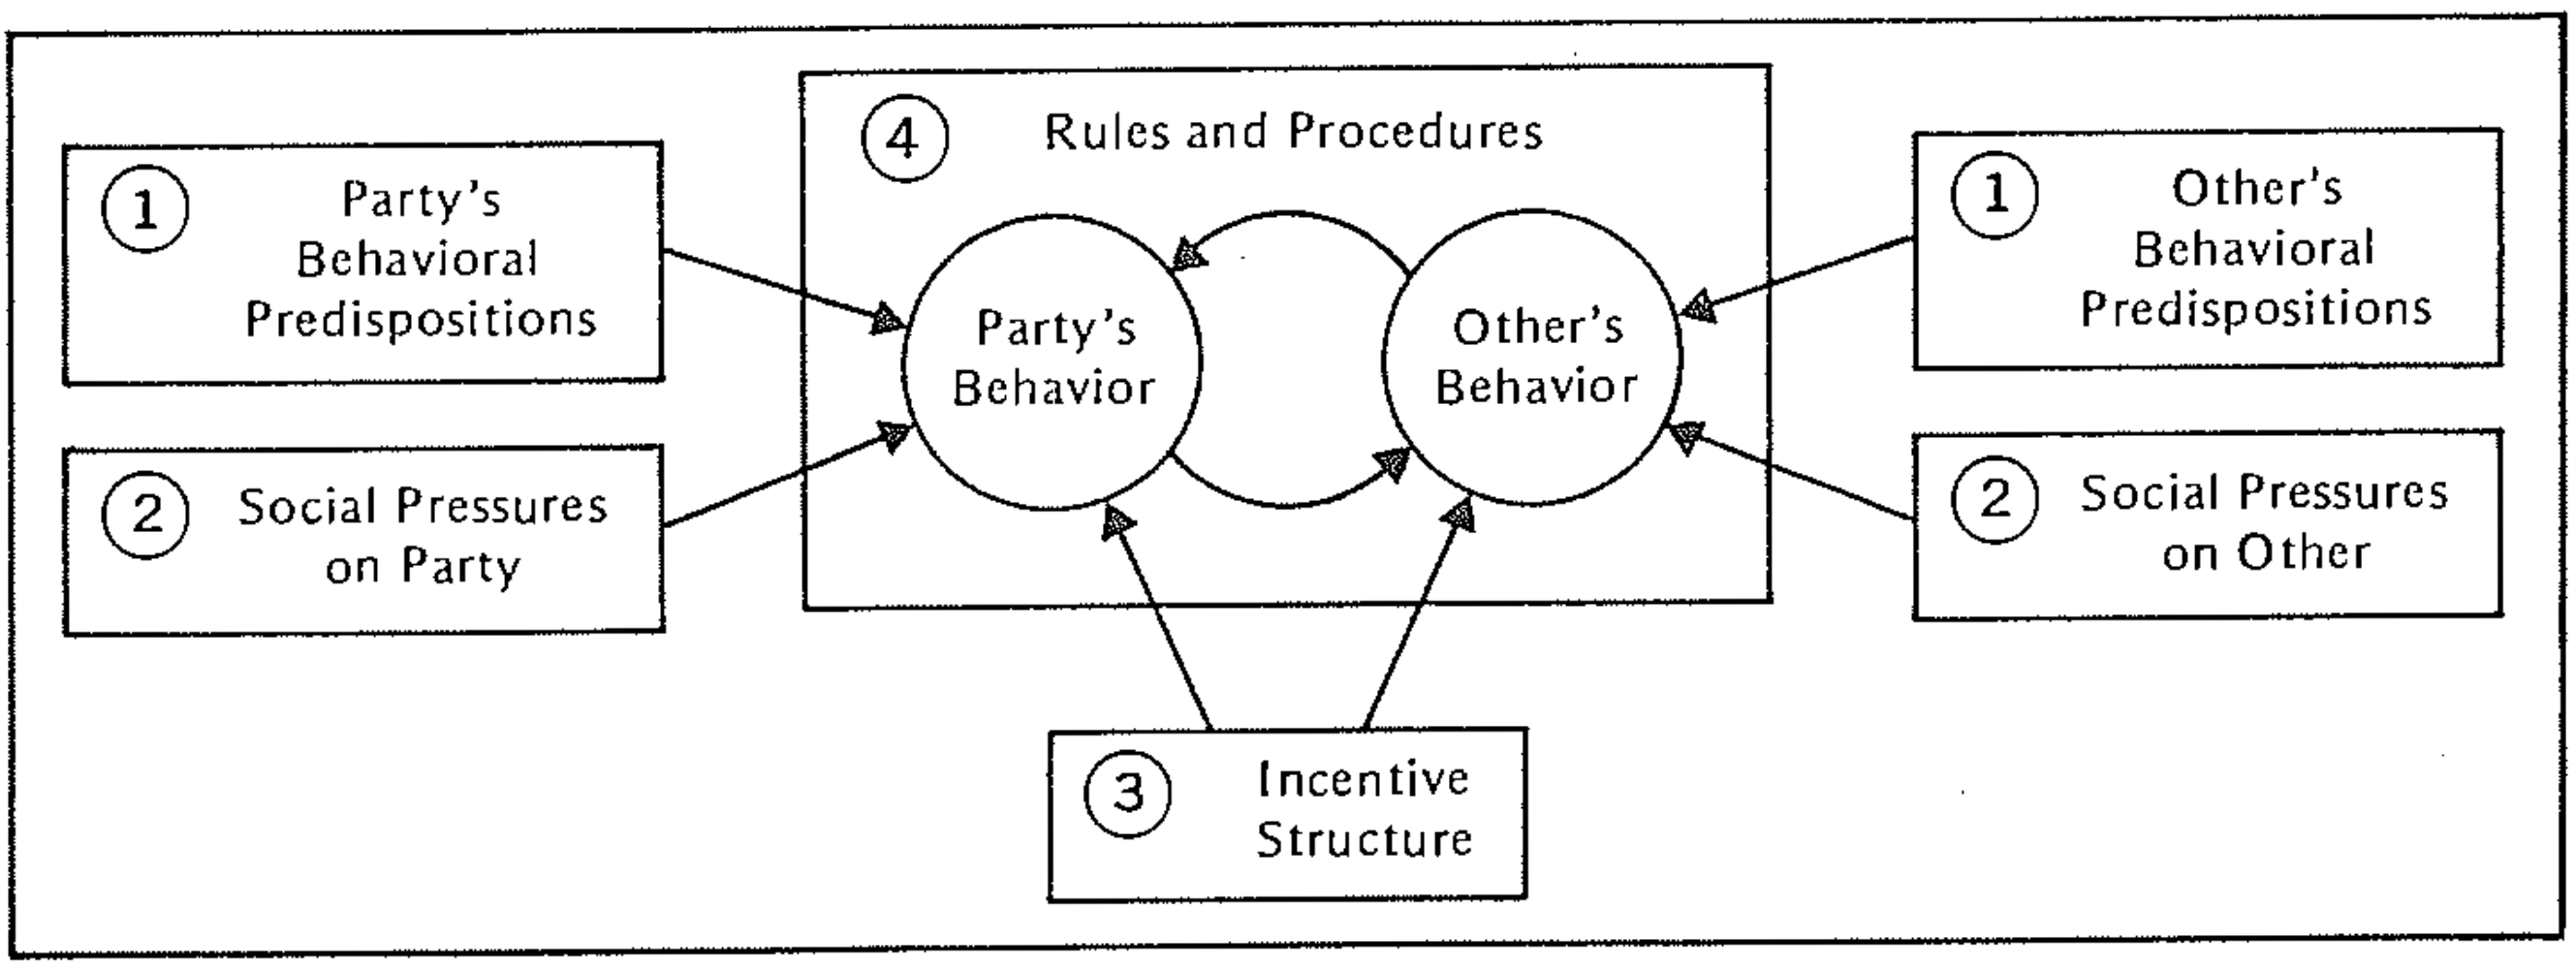
\includegraphics[width=1.0\textwidth]{images/structural_model.png}
%	\end{figure}
\end{frame}

\begin{frame}
	\frametitle{Verhaltensabsichten}
	\begin{itemize}
		\item Dominanter Stil: Prim\"arziel, dass erreicht werden soll
		\item Backup Stil: Falls das Prim\"arziel nicht erreicht werden kann werden alternative Ziele verfolgt
	\end{itemize}
\end{frame}

\begin{frame}
	\frametitle{Sozialer Druck}
	\begin{itemize}
		\item Druck des Auftraggebers\,/\,der repr\"asentierten Gruppe
		\item Umgebender sozialer Druck durch neutrale Beobachter oder kulturelle Werte 
	\end{itemize}
\end{frame}

\begin{frame}
	\frametitle{Beziehung zwischen den Interessen der Parteien}
	\begin{itemize}
		\item Abh\"angig davon, ob ein Interessenkonflikt vorliegt
		\begin{itemize}
			\item Wettbewerb: Knappe Ressourcen erm\"oglichen nur die Umsetzung der Interessen einer Partei
			\item Gemeinsame Probleme: F\"ordert kooperatives Verhalten
			\item Kombination aus beiden
		\end{itemize}
	\end{itemize}
\end{frame}

%//============== F�hrungsstile

\section{F�hrungsstile}
\begin{frame}
	\frametitle{F�hrungsstile}		
	\begin{itemize}
		\pause
		\item Vermeidung \textcolor{lightgray}{(in-action)}			% Robin
		\pause
		\item Machteinsatz \textcolor{lightgray}{(contending)}		% Sven
		\pause
		\item Anpassung \textcolor{lightgray}{(with-drawing)}		% Robin
		\pause
		\item Kompromiss \textcolor{lightgray}{(compromising)}		% Sven
		\pause
		\item Zusammenarbeit \textcolor{lightgray}{(problem solving)}	% Sven
		\pause
	\end{itemize}
\end{frame}

\begin{frame}
	\frametitle{5-Punkte-Modell\,/\,Diagramm}
% TODO: Temporary removed. Include in final again!!! (Sven)
\begin{center}$<$BILD: 5-Punkte-Diagramm$>$\end{center}
%	\begin{figure}[p]
% 		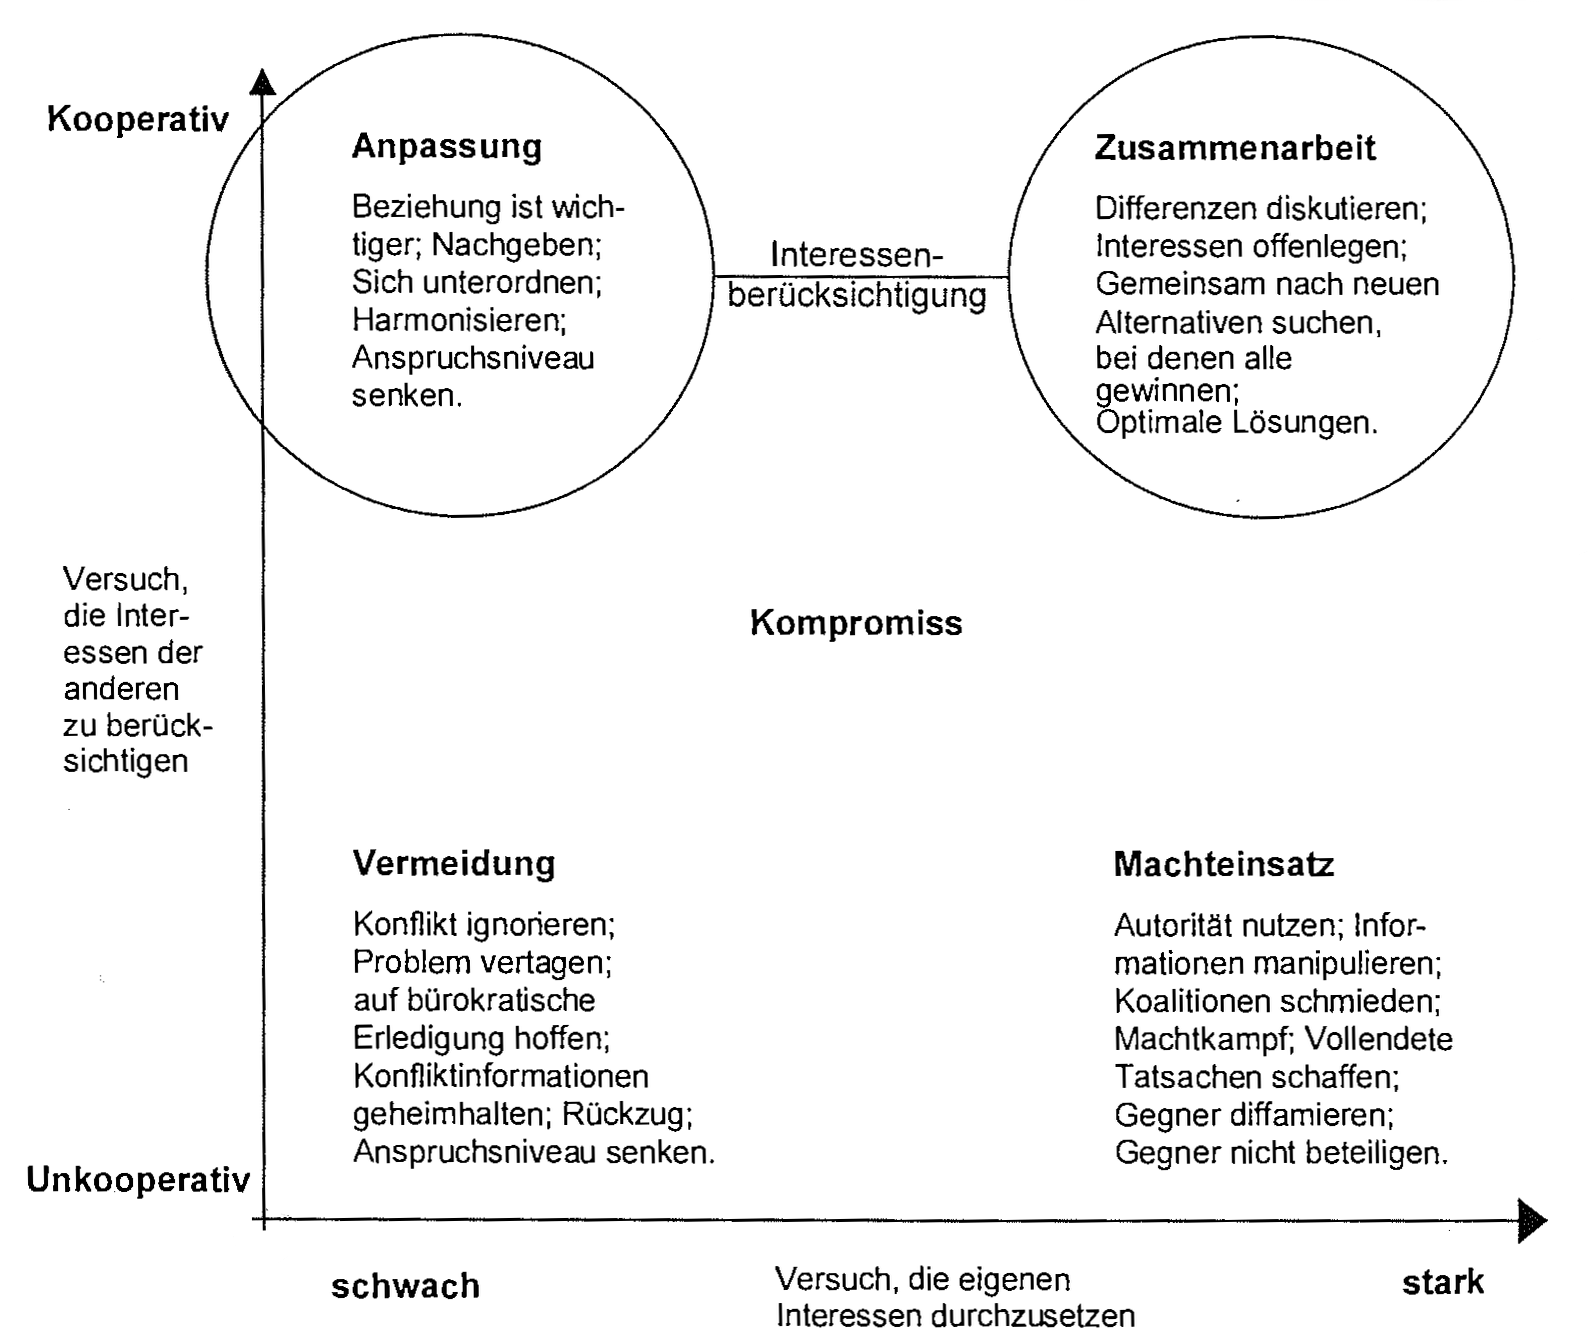
\includegraphics[width=0.8\textwidth]{images/konflikthandhabungsstile.png}
%		%\caption{Meine Abbildung, untertitel}
%	\end{figure}
\end{frame}

\subsection{Vermeidung}
\begin{frame}
	\frametitle{Vermeidung}
	\begin{itemize}
		\item Konflikte werden ignoriert
		\item Bei Konfrontation: Flucht
		\item Unterscheidung von kurz- und langfristiger Vermeidung
	\end{itemize}
\end{frame}

\subsection{Machteinsatz}
\begin{frame}
	\frametitle{Machteinsatz}
	\begin{itemize}
		\item Saktionen
		\begin{itemize}
			\item positiv
			\item negativ
		\end{itemize}
		\item Legitime Anspr�che
		\item �berzeugende Informationen
	\end{itemize}
\end{frame}

\begin{frame}
	\frametitle{Indirekter Machteinsatz}
	Zeichnet sich durch \textbf{Vermeidung} direkter Konfrontation aus.
	\begin{itemize}
		\pause
		\item B�rokratie
		\item Ver�nderung der Regeln
		\item Hinter anderer R�cken
		\item Allianzen
		\item Passiver Widerstand
		\pause
		\begin{itemize}
			\item \emph{Negativismus}: K�rpersprache, knappe Verbalisierung
			\item \emph{Konformit�t}: Skala von unkooperativ ... (geheime) Sabotage
			\item \emph{Mauern}: keine Kommentare, keine Handlung
		\end{itemize}
%		\begin{description}
%			\item[Negativismus] K�rpersprache, knappe Verbalisierung
%			\item[Konformit�t] Skala von unkooperativ ... (geheime) Sabotage
%			\item[Mauern] keine Kommentare, keine Handlung
%		\end{description}
	\end{itemize}
\end{frame}

\begin{frame}
	\frametitle{Direkter Machteinsatz}
	Sehr weites Spektrum, je nach Kontext.
	\begin{enumerate}
	%\setcounter{enumi}{4}
		\item<+->{Offen}
		\begin{itemize}
			\item Anschreien, schupsen, streiken, schlagen, Dinge werfen, ...
			\item An-\,/\,Auslachen des Gegen�bers
			\item (falsche) Behauptungen aufstellen, Beschuldigen, Beleidigen, ...
		\end{itemize}
		\item<+->{Privat}
		\begin{itemize}
			\item Einschmeicheln
			\item \emph{�berzeugende} Argumentation 
			\item In Verlegenheit bringen
			\item Versprechungen machen
			\item ...
		\end{itemize}
		\item<+->{�ffentlich}
		\begin{itemize}
			\item \glqq{}Whistle-Blowing\grqq{}
			\item Gericht
			\item Presse
		\end{itemize}
	\end{enumerate}
\end{frame}

\begin{frame}
	\frametitle{Fairer Machteinsatz}
	Beide Parteien erkennen (in stiller �bereinkunf) bestimmte Regeln an.
	\pause
	\begin{itemize}
		\item z.\,B. im Sport
	\end{itemize}
\end{frame}

\subsection{Anpassung}
\begin{frame}
	\frametitle{Anpassung}
	\begin{itemize}
		\item Erf�llung der W�nsche der anderen Partei ohne Ri�cksicht auf eigene Interessen
		\item Kann verschiedene Gr�nde haben
		\begin{itemize}
			\item Akzeptanz der (fachlichen) �berlegenheit der anderen Partei
			\item Aufbau von sozialem Kredit
			\item Gesichtswahrung bei Hinzuziehen eines Mediators
		\end{itemize}
	\end{itemize}
\end{frame}

\subsection{Kompromiss}
\begin{frame}
	\frametitle{Kompromiss}
	\begin{itemize}
		\item Mischung aus den F�hrungsstilen
		\begin{itemize}
			\item Vermeidung
			\item Anspassung
			\item Machteinsatz
		\end{itemize}
		\pause
		\item Vorgehen daher Summe bzw. ganz �hnlicher der zuvor gen. Stile
		\begin{itemize}
			\item Feilschen, Drohen, K�mpfen, Einlenken, ...
		\end{itemize}
	\end{itemize}
	\pause
	\vspace{8pt}
	$\curvearrowright$ \emph{Brauchbare statt opt. L�sung.}
\end{frame}

\subsection{Zusammenarbeit}
\begin{frame}
	\frametitle{Zusammenarbeit}
	\begin{itemize}
		\item offene Verhandlung
		\item Kreativit�t
		\item Inovativit�t
	\end{itemize}
	\vspace{8pt}
	$\curvearrowright$ \emph{\underline{neue} L�sungen finden -- statt in alten Strukturen verharren.}
\end{frame}

\begin{frame}
	\frametitle{Erreichen von Zusammenarbeit}
	Dies ist in der Regel sehr schwer, da Zusammenarbeit Vertrauen bedingt.
	\pause
	\begin{itemize}[<+->]
		\item Neue Informationen
		\item Dritte Partei
		\item Mediator
	\end{itemize}
\end{frame}

%//Optional
\section{Zusammenfassung}
\begin{frame}
	\frametitle{Zusammenfassung der Modelle}
	\begin{itemize}
		\item Prozessmodell
		\begin{itemize}
			\item Beschreibt interne Dynamik eines Konfliktes als Ablauf von Phasen
			\item Phasen bilden abh\"angige Eventzyklen
		\end{itemize}
		\item Strukturmodell
		\begin{itemize}
			\item Beschreibt intern einen Konflikt als Mischung von Druck und Interessen von verschiedenen Parteien
		\end{itemize}
	\end{itemize}
\end{frame}

\begin{frame}
	\frametitle{Quellen}
	\begin{thebibliography}{9}
		\bibitem[Priutt]{priu} \textit{Priutt Robin, 1986}
		\bibitem[Scholl]{scholl} \textit{Scholl, 2004}
		\bibitem[Thomas]{thom} \textit{Thomas, 1976}
		\bibitem[Vliert]{van} \textit{van de Vliert, 1994}
	\end{thebibliography}
\end{frame}

\end{document}
